\documentclass[11pt, a4paper]{article}
%\usepackage{proj1}
\usepackage{natbib}
\usepackage{fancyhdr}  
\usepackage{subcaption}
\usepackage{caption}
\usepackage{graphicx}
\linespread{1.25} 
\setlength{\parindent}{0cm}
\graphicspath{{Images/}}
\usepackage{hyperref}
\usepackage{amsmath}
\usepackage{amsfonts}
\usepackage{amssymb}
\usepackage{amsthm}
\usepackage{mathtools}
\usepackage{commath}

%\usepackage[sc,osf]{mathpazo}
\usepackage{subcaption}
\usepackage[a4paper, top=1in, left=1.0in, right=1.0in, bottom=1in, includehead, includefoot]{geometry} %Usually have top as 1in

\usepackage{listings}
\usepackage{color} %red, green, blue, yellow, cyan, magenta, black, white
\definecolor{mygreen}{RGB}{28,172,0} % color values Red, Green, Blue
\definecolor{mylilas}{RGB}{170,55,241}


\hypersetup{colorlinks,linkcolor={black},citecolor={blue},urlcolor={black}}
\usepackage{color}
\urlstyle{same}


\theoremstyle{definition}
\newtheorem{definition}{Definition}[section]

\title{Exact Solutions for the Full Problem \\with Force Control and with Flow Control}
\date{}
\newcommand{\Sta}{\rho}
\newcommand{\Adj}{p}
\newcommand{\Con}{u}

\pagenumbering{gobble}
\begin{document}

\section{Perturbation Functions}
We consider the following two perturbation functions, normalised to a maximum of 1. They both originate from the function:
\begin{align*}
f(t) = \frac{e^{-a/t}}{e^{-a/t} + e^{-a/(1-t)}}.
\end{align*}

The first perturbation is in time only and is defined as:
\begin{align*}
g(t) &= \frac{1}{2} f(t-t_0, a) \times f(t-t_0, -a)\\
     &= \frac{1}{2} \frac{e^{-a/(t-t_0)}}{e^{-a/(t-t_0)} + e^{-a/(1-t -t_0)}} \times \frac{e^{a/(t-t_0)}}{e^{a/(t-t_0)} + e^{a/(1-t - t_0)}}.
\end{align*}
The normalised version is then 
\begin{align*}
\tilde g(t) = \frac{g(t)}{\max{\abs{g(t)}}},
\end{align*}
so that $\max{\tilde g(t)} =1$.
With $a = 0.7$ and $t_0 = -0.01$, this looks like Figure \ref{Perttime1} (left).
\begin{figure}[h]
	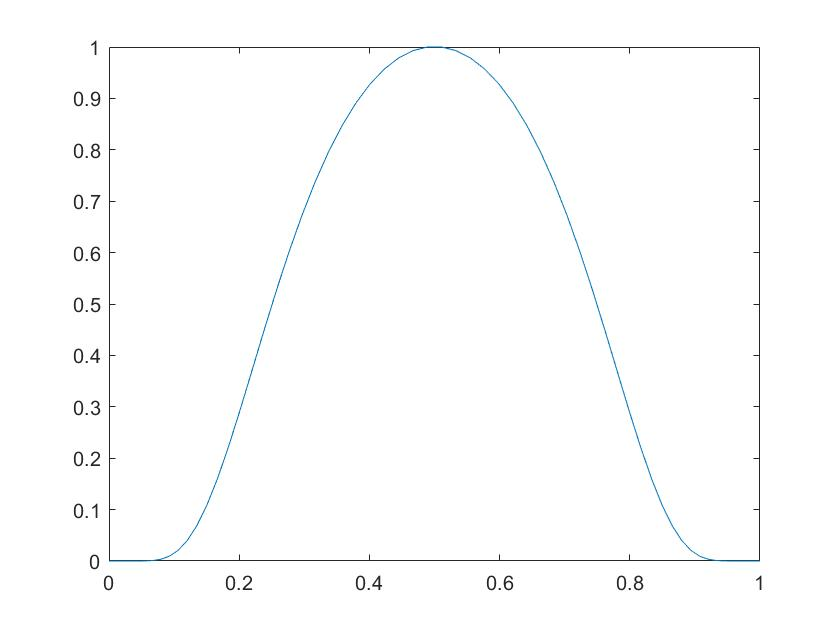
\includegraphics[scale=0.3]{Perttime1.jpg}
	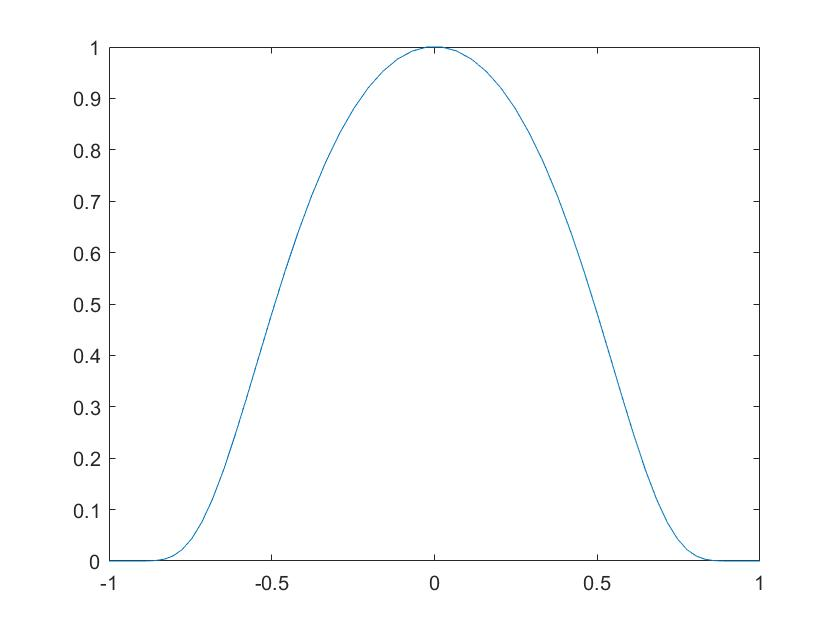
\includegraphics[scale=0.3]{Perttimespace1.jpg}
	\caption{Perturbation $\tilde g(t)$ (left) and $\tilde h(x)$ (right) with $a =0.7$ and $t_0 = -0.01$.}
	\label{Perttime1}
\end{figure}

A similar perturbation can be done in space:
\begin{align*}
h(x) &= \frac{1}{2} f(x-x_0, 2a) \times f(x-x_0, -2a)\\
&= \frac{1}{2} \frac{e^{-2a/(x-x_0)}}{e^{-2a/(x-x_0)} + e^{-2a/(1-x-x_0)}} \times \frac{e^{2a/(x-x_0)}}{e^{2a/(x-x_0)} + e^{2a/(1-x-x_0)}}.
\end{align*}
Again, the normalised version is then 
\begin{align*}
\tilde h(x) = \frac{h(x)}{\max{\abs{h(x)}}}.
\end{align*}
With $a = 0.7$ and $t_0 = -0.01$, this looks like Figure \ref{Perttime1} (right).
\\
The considered perturbations are applied as follows:
\begin{align*}
w_{pert} &= w_{ex}(1+ \epsilon \tilde g(t))\\
w_{pert} &= w_{ex}(1+ \epsilon \tilde g(t) \tilde h(x)).
\end{align*}
The perturbations considered below are all with $\epsilon = 1$, however, when testing convergence, $\epsilon$ will be varied.\\
Applying the time perturbation to Neumann (plus2, $e^t$) Flow Control, the error in $w$ is up to $25$, see Figure \ref{Perttime2}. For the Dirichlet Case ($e^t$), the maximum error in $w$ with the same perturbation is $3$.
\begin{figure}[h]
	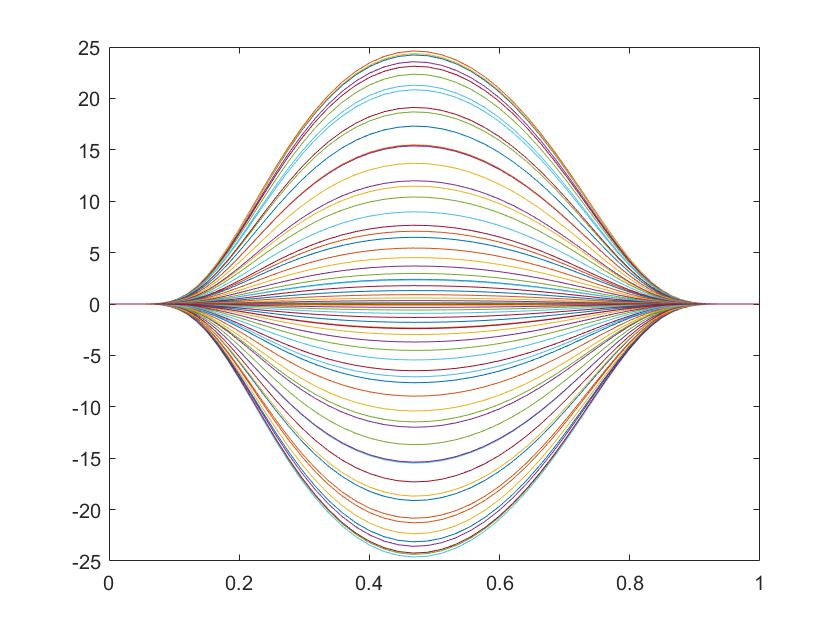
\includegraphics[scale=0.3]{PerttimeN1.jpg}
	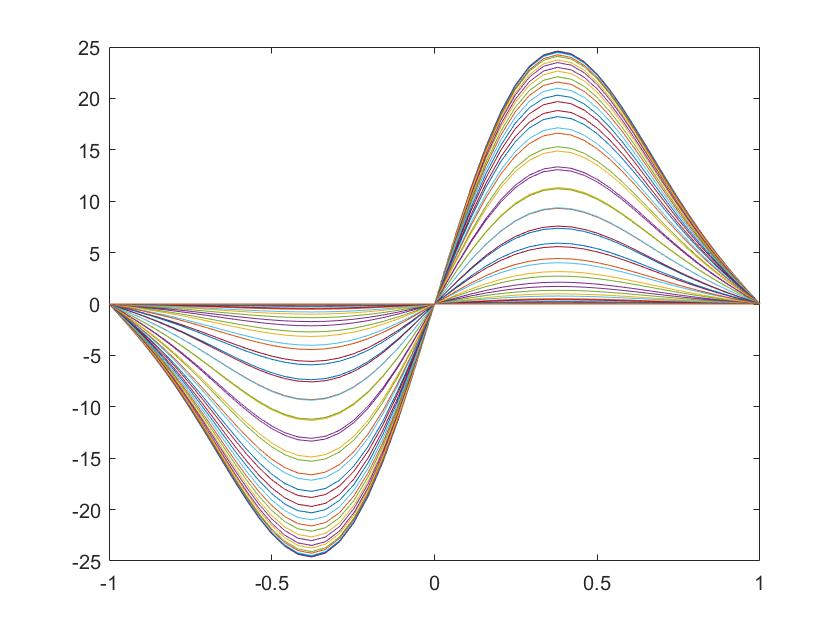
\includegraphics[scale=0.3]{PerttimeN2.jpg}
	\caption{Error in $w$ (Neumann plus2 $e^t$) due to $\tilde g(t)$, with $a =0.7$ and $t_0 = -0.01$.}
	\label{Perttime2}
\end{figure}
\begin{figure}[h]
	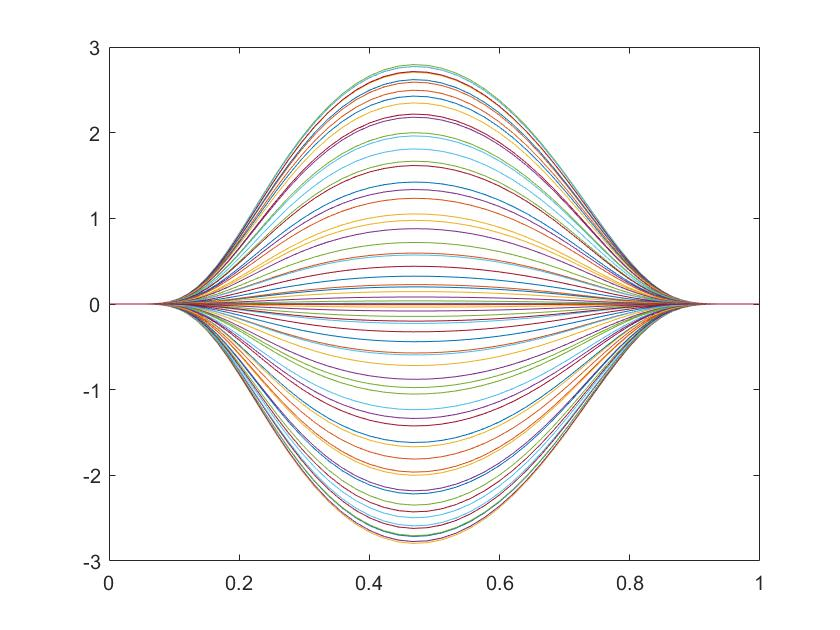
\includegraphics[scale=0.3]{PerttimeD2.jpg}
	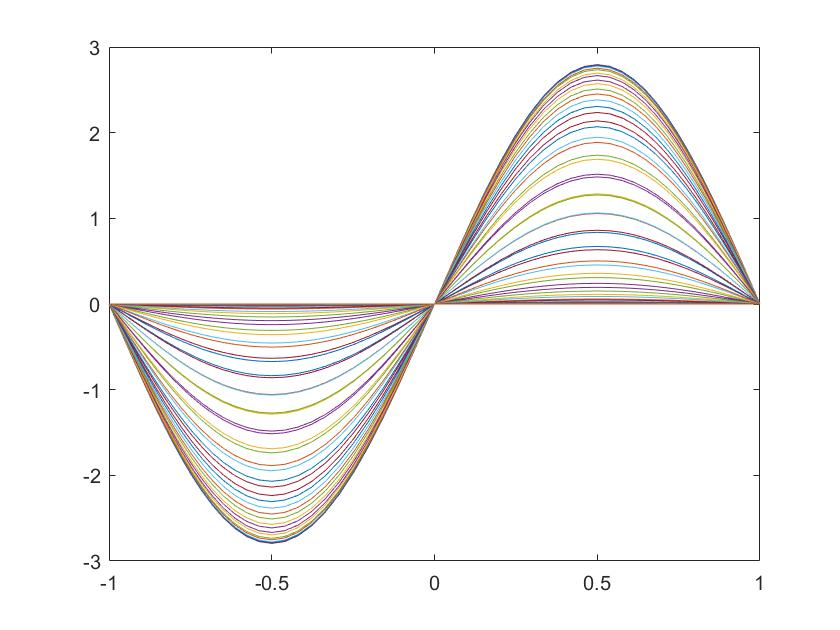
\includegraphics[scale=0.3]{PerttimeD1.jpg}
	\caption{Error in $w$ (Dirichlet $e^t$) due to $\tilde g(t)$, with $a =0.7$ and $t_0 = -0.01$.}
	\label{Perttime3}
\end{figure}
When choosing the linear in time Neumann (plus 2) problem, the maximum error of the same perturbation, $\tilde g(t)$, is $1.8$, see Figure \ref{Perttime5}.
For the linear in time Dirichlet problem, the maximum error is only $0.4$ for the same perturbation, see Figure \ref{Perttime4}.
\begin{figure}[h]
	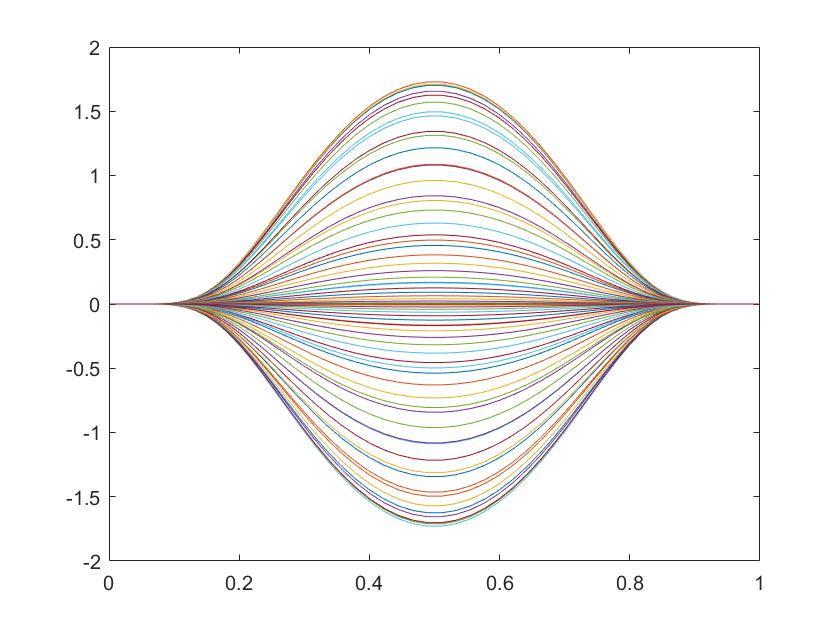
\includegraphics[scale=0.3]{PerttimeN3.jpg}
	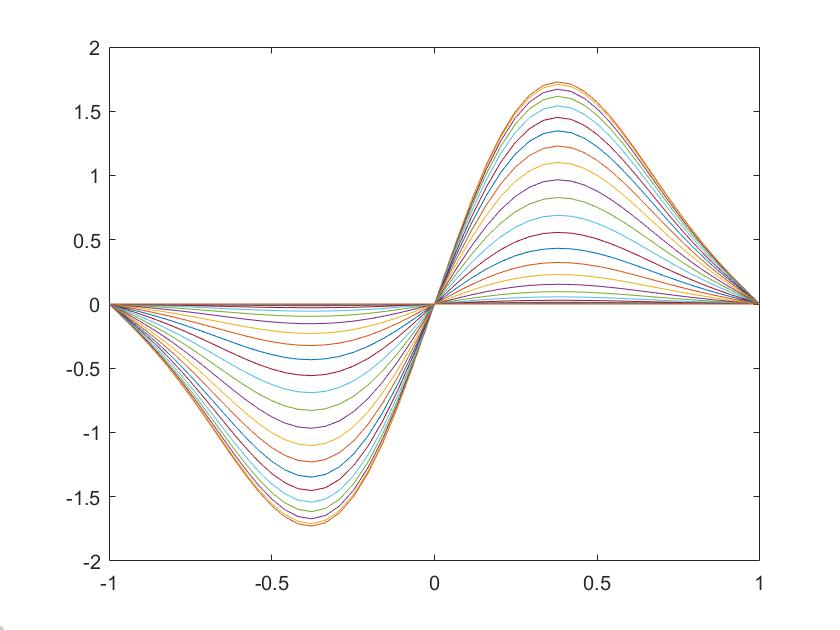
\includegraphics[scale=0.3]{PerttimeN4.jpg}
	\caption{Error in $w$ (Neumann plus2, linear $t$) due to $\tilde g(t)$, with $a =0.7$ and $t_0 = -0.01$.}
	\label{Perttime5}
\end{figure}

\begin{figure}[h]
	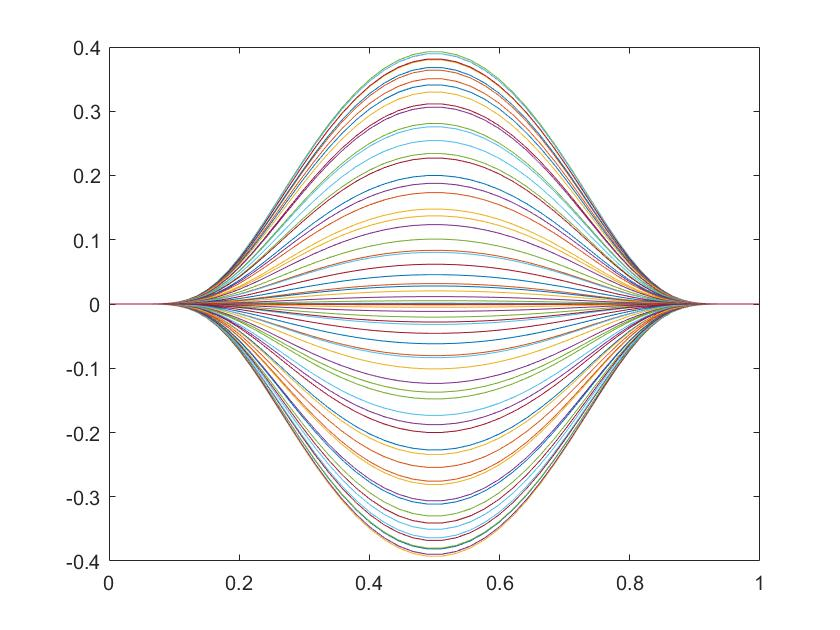
\includegraphics[scale=0.3]{PerttimeD3.jpg}
	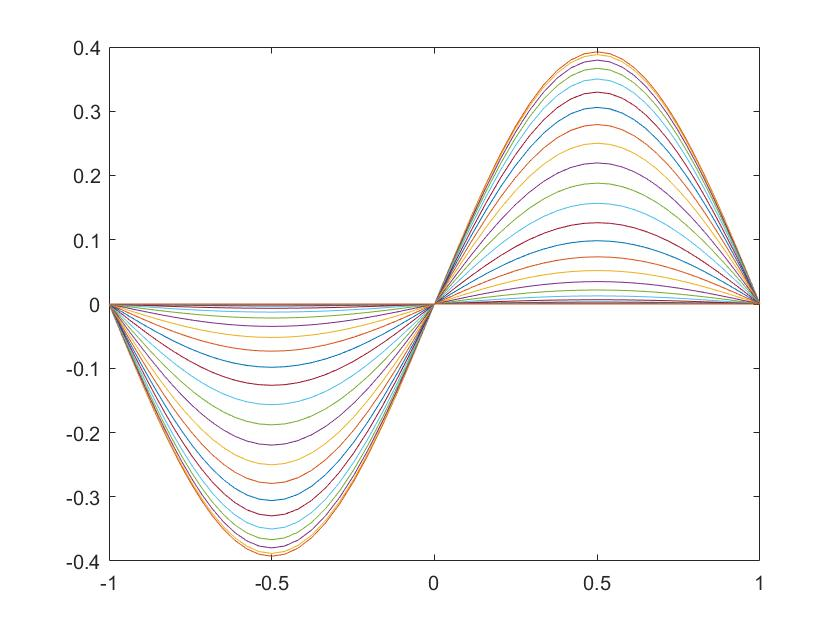
\includegraphics[scale=0.3]{PerttimeD4.jpg}
	\caption{Error in $w$ (Dirichlet, linear $t$) due to $\tilde g(t)$, with $a =0.7$ and $t_0 = -0.01$.}
	\label{Perttime4}
\end{figure}

\begin{figure}[h]
	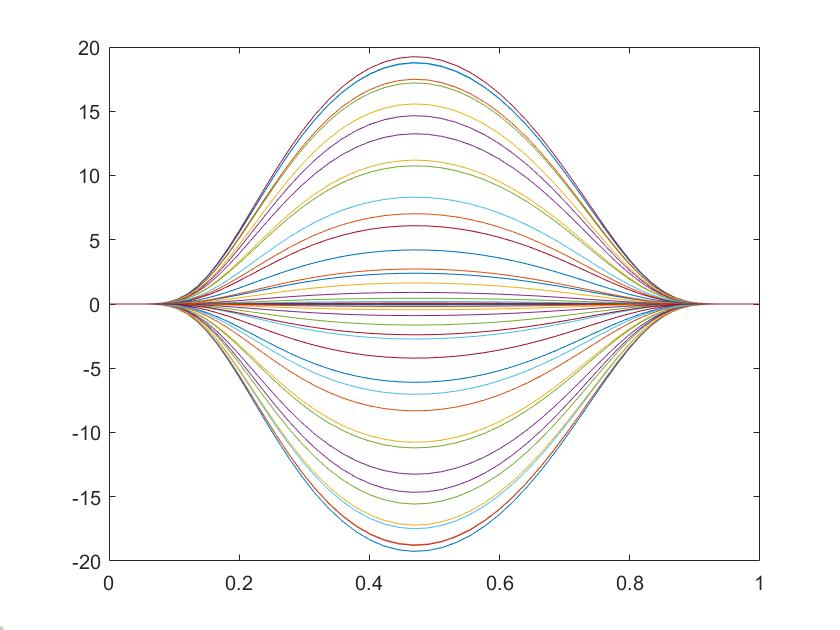
\includegraphics[scale=0.3]{PerttxN1.jpg}
	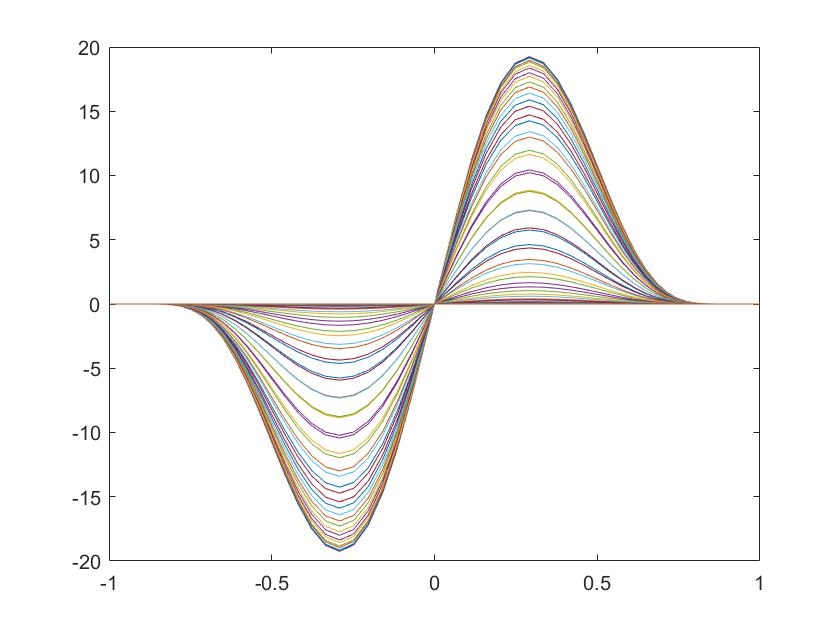
\includegraphics[scale=0.3]{PerttxN2.jpg}\\
	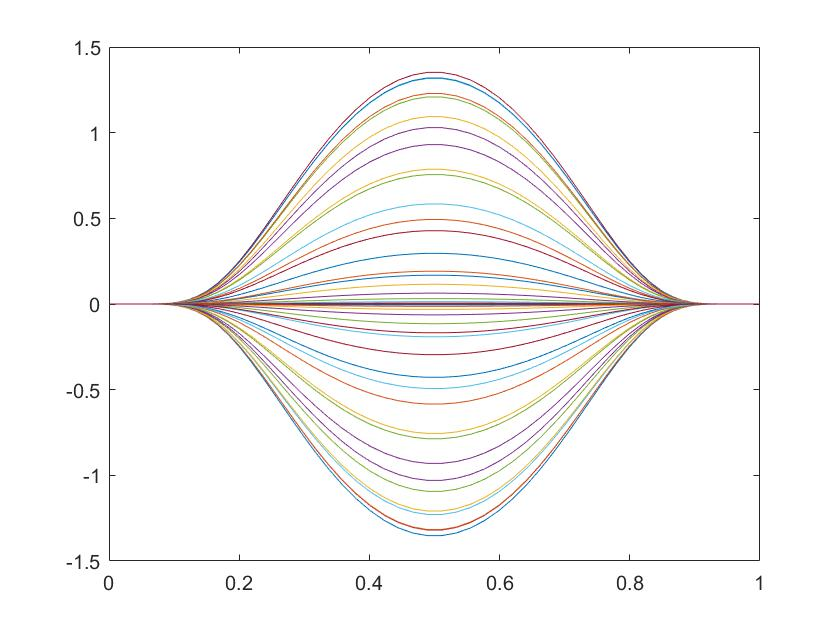
\includegraphics[scale=0.3]{PerttxN3.jpg}
	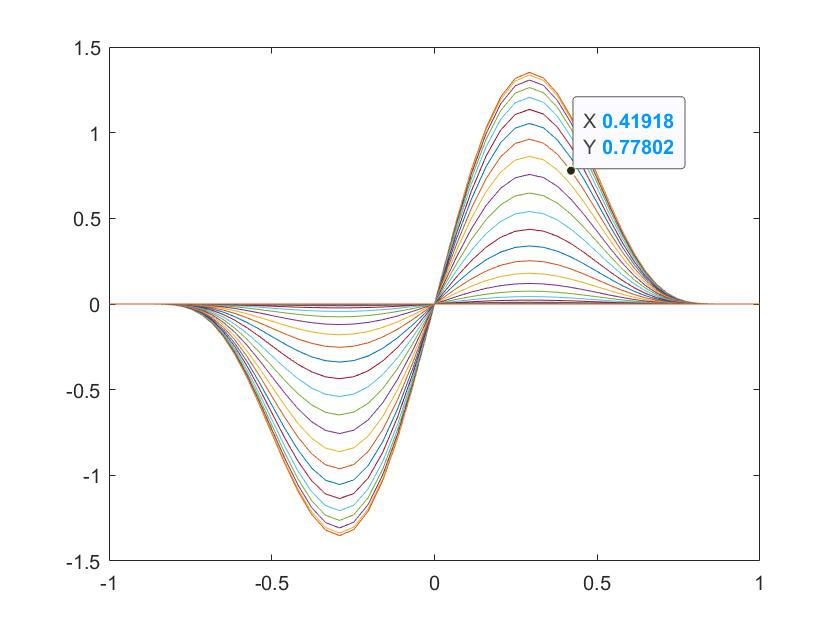
\includegraphics[scale=0.3]{PerttxN4.jpg}
	\caption{Error in $w$ (Neumann plus2) due to $\tilde g(t) \tilde h(x)$, top $e^t$, bottom linear $t$, with $a =0.7$ and $t_0 = -0.01$.}
	\label{Perttx1}
\end{figure}
\begin{figure}[h]
	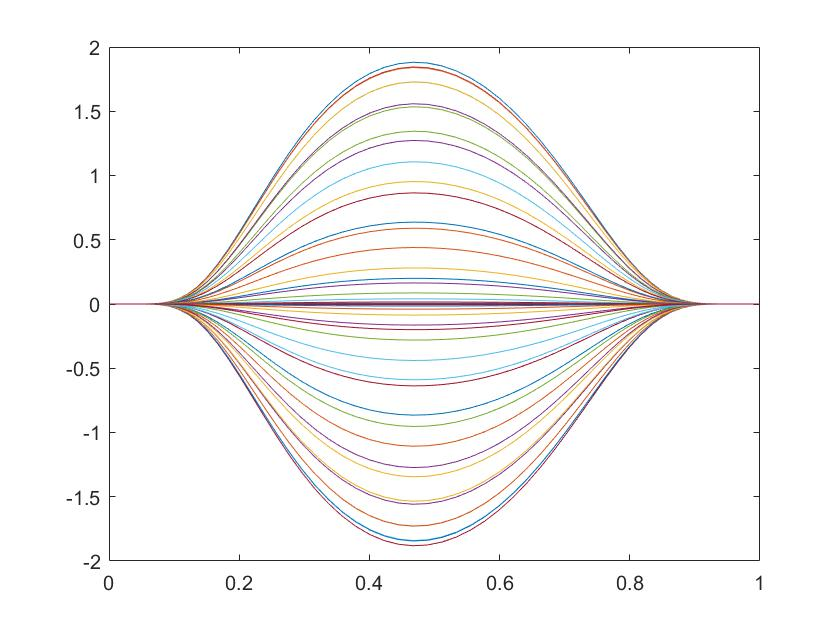
\includegraphics[scale=0.3]{PerttxD1.jpg}
	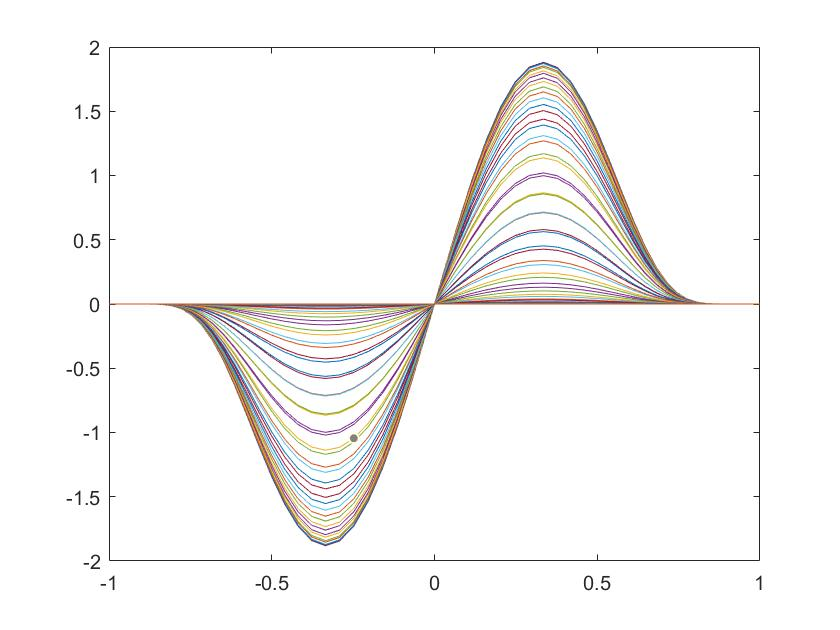
\includegraphics[scale=0.3]{PerttxD2.jpg}\\
	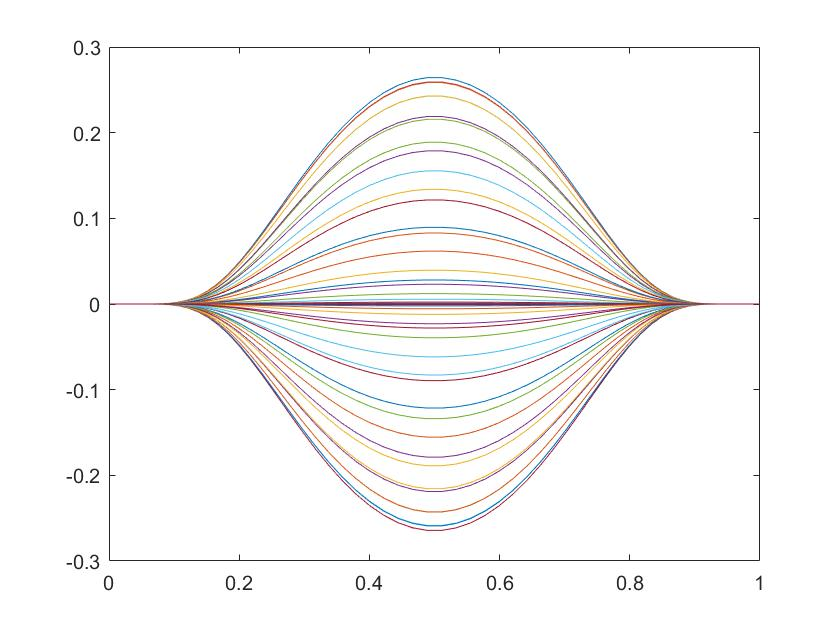
\includegraphics[scale=0.3]{PerttxD3.jpg}
	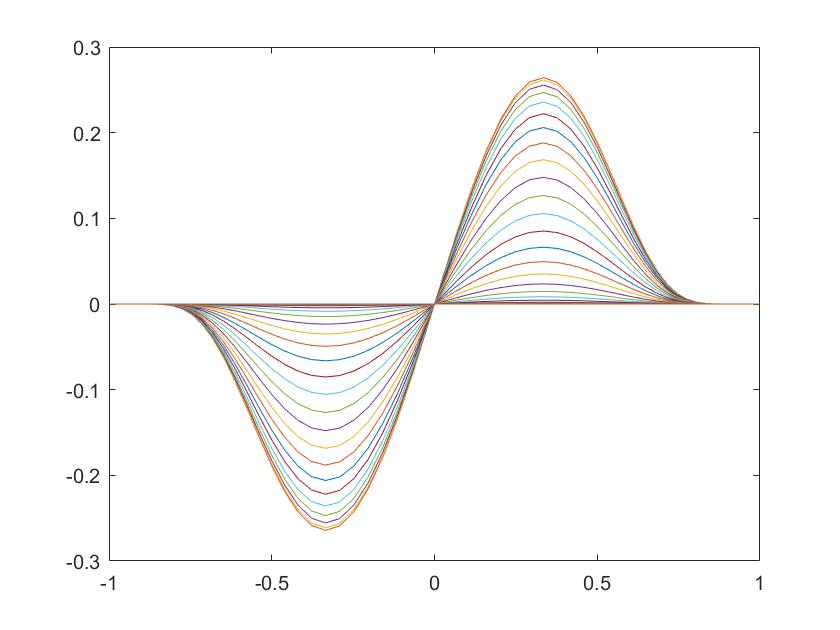
\includegraphics[scale=0.3]{PerttxD4.jpg}
	\caption{Error in $w$ (Dirichlet) due to $\tilde g(t) \tilde h(x)$, top $e^t$, bottom linear $t$, with $a =0.7$ and $t_0 = -0.01$.}
	\label{Perttx2}
\end{figure}
When perturbing in time and space with $\tilde g(t) \tilde h(x)$, Figure \ref{Perttx1} shows that with Neumann (plus2) and $e^t$ the maximum magnitude of the error is lowered from $25$ to $20$, and for linear $t$ from $1.8$ to $1.5$.
In Figure \ref{Perttx2}, similar observations can be made for the Dirichlet case. In the $e^t$ case, the maximum error decreases from $3$ to $2$ and in the linear $t$ case from $0.4$ to $0.3$.




\end{document}